\documentclass[bsc,en]{ufpethesis}

\usepackage[ruled]{algorithm2e}
\SetKwInOut{Input}{Input}\SetKwInOut{Output}{Output}
\usepackage{algpseudocode}
\usepackage{amsmath}
\usepackage{xspace}
\usepackage{xcolor}
\usepackage{setspace}
\doublespacing
\usepackage{lineno}
\usepackage{outlines}
\usepackage[normalem]{ulem}
\usepackage{paralist}
\usepackage{graphicx}
\usepackage{caption}
\usepackage{subcaption}


\newcommand{\prob}{\ensuremath{\mathrm{Pr}}}
\newcommand{\dB}{de~Bruijn\xspace}
\newcommand{\dBG}{de~Bruijn graph\xspace}
\newcommand{\dBCM}{DBCM\xspace}
\newcommand{\dBHT}{DBHT\xspace}
\newcommand{\cm}{CountMin\xspace}
\newcommand{\kmer}{\mbox{$k$-mer}\xspace}
\newcommand{\chr}[1]{\ensuremath{\mathtt{#1}}}
\newcommand{\A}{\chr{A}}
\newcommand{\C}{\chr{C}}
\newcommand{\G}{\chr{G}}
\newcommand{\T}{\chr{T}}
\newcommand{\keyterm}[1]{\textit{\textbf{#1}\/\xspace}}
\newcommand{\str}[2]{\ensuremath{#1_0\cdots#1_{#2-1}}}
\newcommand{\strname}[1]{\ensuremath{\uppercase{#1}}}
\newcommand{\strdef}[2]{\ensuremath{\strname{#1}=\str{#1}{#2}}}
\newcommand{\strslice}[3]{\ensuremath{\strname{#1}[#2:#3]}}
\newcommand{\strsetname}[1]{\ensuremath{\mathcal{\uppercase{#1}}}}

\newcommand{\tochange}[1]{\color{red} #1 \color{black}}
\newcommand{\toconsider}[1]{\color{blue} #1 \color{black}}
\newcommand{\asq}[1]{\color{red}$\rightarrow$ asq says: #1 $\leftarrow$ \color{black}}
\newcommand{\paguso}[1]{\color{magenta}$\rightarrow$ paguso says: #1 $\leftarrow$ \color{black}}
\newcommand{\remove}[2][]{\color{magenta}{\sout{#2}(\textit{#1})}\color{black}}
\newcommand{\change}[3][]{\remove[#1]{#2}{#3}}

\newcommand{\readset}{\strsetname{X}\xspace}

\university{Universidade Federal de Pernambuco}
\institute{Centro de Informática}
\program{Bacharelado em Engenharia da Computação}
\majorfield{Engenharia da Computação}

\author{Augusto Sales de Queiroz}

\adviser{Paulo Gustavo Soares da Fonseca}

\title{Space-efficient representation of de~Bruijn graphs for data streams}

\begin{document}
    \linenumbers
    \frontmatter
    \frontpage
    \presentationpage
    \tableofcontents

    \mainmatter
	\linenumbers
	\doublespacing
    \chapter{Introduction}
    \chapter{Related Works}

\section{Outline}

\begin{outline}
    \1 Short-read sequencing
        \2 Sequencing errors
    \1 Assembler Architecture
        \2 \dBG
        \2 Pre-processing of reads
            \3 \kmer counting \& filtering
                \4 khmer\cite{Zhang2014}
    \1 Navigational Data Structures (NDS)
        \2 \cite{Chikhi2014}
    \1 \emph{FastEtch} \cite{Ghosh2019}
        \2 Online counting $\rightarrow$ Filtering $\rightarrow$ Construction of \dBG
\end{outline}

\section{Notation}

Throughout this work, we use lower-case symbols, such as $t$ and $c$, to represent scalar values. Uppercase symbols, such as $\strname{X}$ and $\strname{Y}$, represent strings. Finally, calligraphic uppercase symbols, such as $\readset$, are used to represent sets. Strings and sets are $0$-indexed, and the notation $X[i:j]$ represents the substring of $X$ from position $i$ up to, but not including, position $j$. When used between two string, or a string and a character, $\strname{X} \cdot \strname{Y}$ represents the concatenation of $\strname{X}$ and $\strname{Y}$.

\section{\dBG{s}}
\label{sec:dBG}

% - Detailed explanation of \dBG of a set of DNA sequences
%   - reverse complements
% - How it is going to be used
% - Operations
%   - Insert node
%   - Insert edge
%   - Query node
%   - Query edge / star 
% - Space-efficient representations - that's what we propose

The \keyterm{\dBG of order $k$} of a string \strdef{x}{n}, $G(X;k)=(V,E)$, is defined as the directed graph whose nodes $V$ represent all distinct \kmer{s} (i.e. substrings of length $k$) of \strname{X}, and such that any two nodes representing $(k-1)$-overlapping \kmer{s} are connected by an edge labeled by the last character of the second \kmer. For example if $k=3$ and $X$ contains the substring \chr{ACGT} then the consecutive triplets \chr{ACG} and \chr{CGT} will originate the edge $\chr{ACG}\stackrel{\chr{C}}{\longrightarrow}\chr{CGT}$. Hence the edges $E$ represent all distinct $(k+1)$-mers of $X$. 
% That is, given two nodes on the graph, they each represent a distinct sequence of symbols $S_1$ and $S_2$, and there is an edge between them if and only if the tail of $S_1$ is the head of $S_2$.

In genome sequencing, \dB graphs are used in the assembly process to represent the distinct \kmer{s} in a set \readset of randomly distributed fragments of the source DNA \strname{S}, called \keyterm{reads}, generated by the sequencing machines. The amount and total length of the reads is determined by the \keyterm{coverage} of the sequencing process, i.e. the number of times \strname{S} was cloned and sequenced. Ideally, \strname{S} could be obtained from an Eulerian traversal of $G(\readset, k)$. Unfortunately however, due to sequencing errors and repeats, such a straightforward approach is not feasible, but the \dBG can still be used to produce a collection of partial assemblies, called \keyterm{contigs}, which can then be further combined to form the original genome \cite{Pevzner2001}. Figure~\ref{fig:dbgexample} presents an example of the \dBG in this context.

\begin{figure}[htbp]
	\begin{center}
    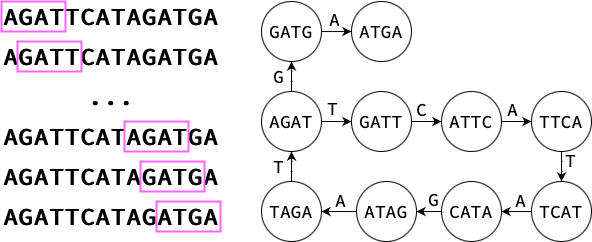
\includegraphics[width=0.8\textwidth]{figures/dbg-example}
	\end{center}
	\caption{Example of a \dBG. $k=4$}\label{fig:dbgexample}
\end{figure}

\subsection{Reverse Complements}
\label{subsec:dBG-reversecomplements}

One difficulty of using \dBG{s} to represent DNA data is the presence of \keyterm{reverse complements}. When generating sequencing reads, the machine reads either of the two complementary strands of a fragment of the input DNA. That is, the output read may correspond to the sequence \strname{S} in the forward (5'-3') direction, or its reverse complement \strname{\overline{S}} in the backward (3'-5') direction, with
\strname{\overline{S}} being obtained from \strname{S} by swapping each base with its Watson-Crick complement
($\A \leftrightarrow \T$, $\C \leftrightarrow \G$) and then reversing the string, and vice versa. For example, the reverse complement of the sequence $S=\chr{AGTACGGTC}$ is $\overline{S}=\chr{GACCGTACT}$ and vice versa.

To deal with reverse complements, reads are processed twice, once in each direction. Nodes representing \kmer{s} that are reverse complements of each other are merged, with edges made bidirectional. Alternatively, those nodes can be kept distinct, resulting in a symmetric graph in which, as noted by Conway \& Bromage, ``a forward traversal corresponds to the backwards traversal on the reverse complement path, and vice versa.'' \cite{Conway2011}
% As in \cite{Conway2011}, this will be treated by processing
% all reads in both directions, without, however, merging nodes representing reverse complements. As noted by Conway \& Bromage: ``This
% makes the graph symmetric; a forward traversal corresponds to a backwards traversal on the reverse complement path, and vice versa.``
% \cite{Conway2011}

\subsection{Selecting the \kmer{s} for the \dBG}
\label{subsec:dBG-selectingkmers}

Another difficulty of using a \dBG to represent DNA data is dealing with sequencing errors. During the sequencing process, there is a small error rate associated with reading any base from \strname{S} (0.1\%--1\% per base in Illumina \cite{Metzker2010}). As a result, many of the \kmer{s} extracted from the reads in \readset are erroneous. As discussed by Conway \& Bromage, this causes the number of spurious \kmer{s} to grow proportionally to the number of bases in the reads $|\readset|=\sum_{\strname{X}_i \in \readset} |\strname{X}_i|$, determined by the coverage, while the number of true \kmer{s} is proportional to the size of the genome $|\strname{S}|$ \cite{Conway2011}.

Although modern sequencing machines generate a quality score associated with each base, it is not possible to know exactly what parts of the reads are erroneous, and so we cannot tell whether a \kmer should be added to the \dBG without more information. However, real \kmer{s} are expected to appear a number of times close to the sequencing coverage $c$, or a multiple of $c$ in case of repeats, whereas spurious \kmer{s} resulting from sequencing errors are commonly low-frequency or even unique \cite{Conway2011, Zhang2014, Ghosh2019}. As such, a natural way of filtering the \kmer{s} obtained from the reads is to discard those that have a low frequency. Hence we consider a \kmer to be a real \kmer iff it occurs more than some threshold $t$, in which case added to the \dBG.

Counting \kmer{s} in a set of reads in a time- and space-efficient manner is, in itself, a challenging task, which is commonly performed as a preprocessing step to the \dBG construction \cite{Zhang2014}. Some assemblers, however, introduce \kmer counting as a part of the \dBG construction, such as the \emph{FastEtch} assembler, which uses a \cm sketch (discussed in Section~\ref{sec:countmin}) to do so \cite{Ghosh2019}.

\subsection{\dBG representation}
\label{subsec:dBG-representation}

A \dBG can be represented either by its set of nodes (\kmer{s}) or edges ($(k+1)$-mers) equivalently, as one can be derived from the other. Therefore, a structure that can determine if a given node $x$ is a member of $G$ can represent the \dBG. Conway \& Bromage showed that the lower bound on the space required to \emph{exactly} represent these \keyterm{membership data structures} (MDS's) is $\Omega(n \log n)$, with $n=|V(G)|$ \cite{Conway2011}.

In order to further improve space-efficiency, new representations were created that trade deterministic exactness for a probabilistic approach. Pel \emph{et al.} showed that a probabilistic representation based on a Bloom Filter could accuratly represent a \dBG with as little as 4~bits per \kmer \cite{Pell2012}.

However, Bowe \emph{et al.} \cite{Bowe2012} and Chikhi \& Rizk \cite{Chikhi2013} independently observed that giving up deterministic exactness isn't the only option for obtaining better space-efficiency, introducing two new representations that use $O(n)$ and $O(n \log k)$ bits, respectively, and allow for an exact traversal of the \dBG from a starting set of known member nodes. This is possible due to the fact that a \dBG is not queried for membership of random nodes, but rather for potential neighbors of nodes already known to be in the graph. As such, the structures designed by the two groups do not offer a deterministically exact membership query operation, instead offering a neighborhood query operation that is exact for the members of the graph \cite{Bowe2012, Chikhi2013}. Chikhi \emph{et al.} later named this new form of representation a \keyterm{Navigational Data Structure} (NDS) and showed that the lower bound on the number of bits required to exactly represent a \dBG with an NDS is $3.24n$ \cite{Chikhi2014}.

Beyond the distinction between probabilistic and exact, and MDSs and NDSs, there is also a distinction between \keyterm{static} and \keyterm{dynamic} representations for \dBG. Static representations are constructed once and never altered, whereas dynamic representations support operations such as insertion and deletion of nodes, useful in population-scale studies due to their everchanging nature \cite{Alipanahi2021}.

% A \dBG can be represented either by its set of nodes (\kmers) or edges ($(k+1)$-mers) equivalently, as one can be derived from the other.
% As such, a structure that can answer queries about the presence of a given node on the graph is enough to
% represent the graph. Conway\&Bromage showed that the lower bound on the space required to
% \emph{exactly} represent a \dBG is $\Omega(n \log n)$ bits, where $n$ is the number of nodes\remove[isn't this obvious?]{,
% and $4^k > n$}\cite{Conway2011}.

% \asq{Isso precisa ser reescrito: NDSs não são necessariamente representações probabilisticas. Elas apenas substituem a consulta de presença de um nó pela consulta de vizinhança.}

% In order to further improve space-efficiency, new representations were created that trade deterministic exactness for a probabilistic approach. For instance, the so-called \keyterm{Navigational Data Structures} (NDS) have some probability of giving an erroneous answer to a membership query, 
% but can still be used to navigate the graph \cite{Chikhi2014}. This \change{definition is useful}{is} due to the fact that a \dBG is usually not queried for membership of \change{randomly selected}{random} nodes, but rather \remove{only} potential neighbors of \change{a known member node is queried}{nodes already known to be in the graph}. In the same paper where they introduce
% the idea of NDS \cite{Chikhi2014}\paguso{correct?}\asq{Esse artigo de Chikhi \emph{et al.} é a introdução e formalização do conceito de NDSs em oposição às Membership Data Structures. Em segunda leitura, porém, categorizar nossas estruturas como NDSs é incorreto porque NDSs devem dar respostas exatas para consultas de vizinhança, o que nós não garantimos.}, Chikhi \emph{et al.} also present a lower bound for the number of bits needed to represent such a structure as $3.24n$.
% In sections \ref{sec:debruijncountmin} and \ref{sec:debruijnhashtable} we will introduce two new NDS's. \asq{É necessário reiterar
% os objetivos das duas estrutas aqui, visto que isso já seria feito na introdução e é feito nas próprias sessões dedicadas a cada estrutura?}\paguso{até o momento, acho que não.}

\subsubsection{Operations}
\label{subsubsec:dbg-operations}

Chikhi \emph{et al.} \cite{Chikhi2019} present the following set of operations common to many data structures for representing a \dBG.

\begin{enumerate}
  \item \emph{Construction} of the data structure
  \item \emph{Insertion} of a new \kmer
  \item \emph{Deletion} of an existing \kmer.
  \item \emph{Membership query}: Given a \kmer $X$, returns true iff $X \in G$
  \item \emph{Forward neighbor query}: Given a \kmer $X$ and a base $a$, returns true iff $X[1:k] \cdot a \in G$
  \item \emph{Backward neighbor query}: Given a \kmer $X$ and a base $a$, return true iff $a \cdot X[0:k-1] \in G$.
\end{enumerate}

Note that a representation that implements the \emph{construction} and \emph{membeship query} operation can use those to implement some version of the others (e.g. by reconstructing the graph with the desired insertion or deletion, or by querying for the membership of the desired neighbor). However, dynamic representations implement \emph{insertion} and \emph{deletion} operations that do not require the reconstruction of the graph, while NDSs don't rely on the membership query to establish if a given forward or backward neighbor is represented in the graph. For example, the neighborhood query described by Chikhi \emph{et al.} \cite{Chikhi2014} as defining NDSs can be implemented by performing \emph{forward} and \emph{backward neighbor queries} for all extensions of the given \kmer and then returning only those for which the result was $\mathit{true}$.
    \chapter{Fundamentação teórica e metodologia}

\section{\dBG}

% - Detailed explanation of \dBG of a set of DNA sequences
%   - reverse complements
% - How it is going to be used
% - Operations
%   - Insert node
%   - Insert edge
%   - Query node
%   - Query edge / star 
% - Space-efficient representations - that's what we propose

The \dBG is a directed graph for which each node represents a sequence of symbols, and each edge between two nodes represents
the overlap between the two sequences. That is, given two nodes on the graph, they each represent a distinct sequence of symbols
$S_1$ and $S_2$, and there is an edge between them if and only if the tail of $S_1$ is the head of $S_2$.

Within the context of genome sequencing, \dB graphs are used in the assembly process by storing the distinct \kmer 's identified
in the read sequences. In the ideal case (when each \kmer is present only once in the original sequence, and there are no
sequencing errors), the complete traversal of this graph would produce the original sequence. In practice, such a straightforward
approach is not feasible, but the \dBG can still be used to produce longer sequences, called \emph{contigs}, which can then be processed
to assemble the original genome. Figure~\ref{fig:dbgexample} presents an example of the \dBG within this context.

\begin{figure}[htbp]
	\begin{center}
    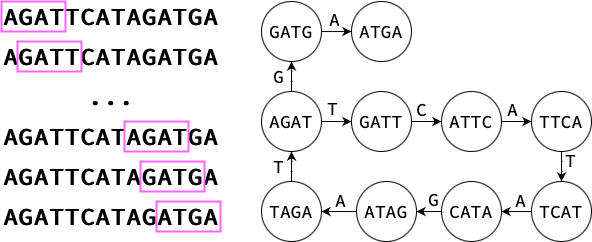
\includegraphics[width=0.8\textwidth]{figures/dbg-example}
	\end{center}
	\caption{Example of a \dBG. $k=4$}\label{fig:dbgexample}
\end{figure}

In a strict definition of a \dBG, the graph must support insertion operations for both nodes and edges. It has long been understood,
however, that storing both node and edge information is redundant, and having only one of the two is sufficient to represent the graph.
In a similar way, the \dBG must allow for the query operation of nodes and edges. In practice, however, only one of these is needed.

\subsection{Reverse Complements}

One individuality of the genome sequencing context is the presence of \emph{reverse complements}. When generating sequencing reads,
a sequence of DNA can be read both in its forward form, or in its reverse complement. That is, the read is generated not from the
original sequence $S$, but its complement $\overline{S}$, generated by swapping each base with its Watson-Crick complement
($\A \leftrightarrow \T$, $\C \leftrightarrow \G$). As in \cite{Conway2011}, this will be treated by processing all reads in both
directions, without, however, merging nodes representing reverse complements. As noted by Conway \& Bromage: ``This makes the graph
symmetric; a forward traversal corresponds to a backwards traversal on the reverse complement path, and vice versa.``\cite{Conway2011}.

\subsection{Representing a \dBG}

Due to its nature, a \dBG can be represented by its set of nodes or edges independently, as one can be derived from the other.
\asq{Citation needed} As such, a structure that can answer queries about the presence of a given node on the graph is enough to
represent the graph. In this regard, Conway \& Bromage showed that a lower bound on the number of bits required to \emph{exactly}
represent a \dBG exists, and is $\Omega(n \log n)$, for $n$ being the number of distinct \kmer's present in the graph, and $4^k > n$
\cite{Conway2011}.

In order to further improve space-efficiency, new forms of representation were created that XXX exactness for a probabilistic approach
such as \emph{Navigational Data Structures} (NDS), which have some probability of giving an erroneous answer to a membership query, 
but can be used to navigate the graph. This definition is useful due to the fact that a \dBG is not queried for the membership of randomly
selected nodes, but rather only the neighborhood of a known member node is queried\cite{Chikhi2014}. In sections \ref{sec:debruijncountmin}
and \ref{sec:debruijnhashtable} we will introduce two new NDS's.

\section{\cm}
\label{sec:countmin}

The \cm sketch, first introduced in \cite{Cormode2005}, is a sub-linear data structure intended to allow for event frequency mapping.
In this way, it must allow for the query of the frequency of a given event, as well as the update of that frequency, through the
\emph{query} and \emph{update} operations. The sketch is composed of a $W$-wide, $D$-deep matrix of counters. With each row in this
matrix is associated a hash function that map the possible events to the $W$ positions in that row, such that all $D$ hash functions
must be pair-wise independent.

Updating the frequency of a given event is done by passing it through the hash functions for each row, and then updating the counter in
the resulting position accordingly.

Querying the structure consists of, similarly, retrieving the value of the counter associated with the key in each row, and then returning
the minimum value among them.

Figure \ref{fig:countminexample} presents a visualization of the \cm sketch.


\begin{figure}[htbp]
	\begin{center}
    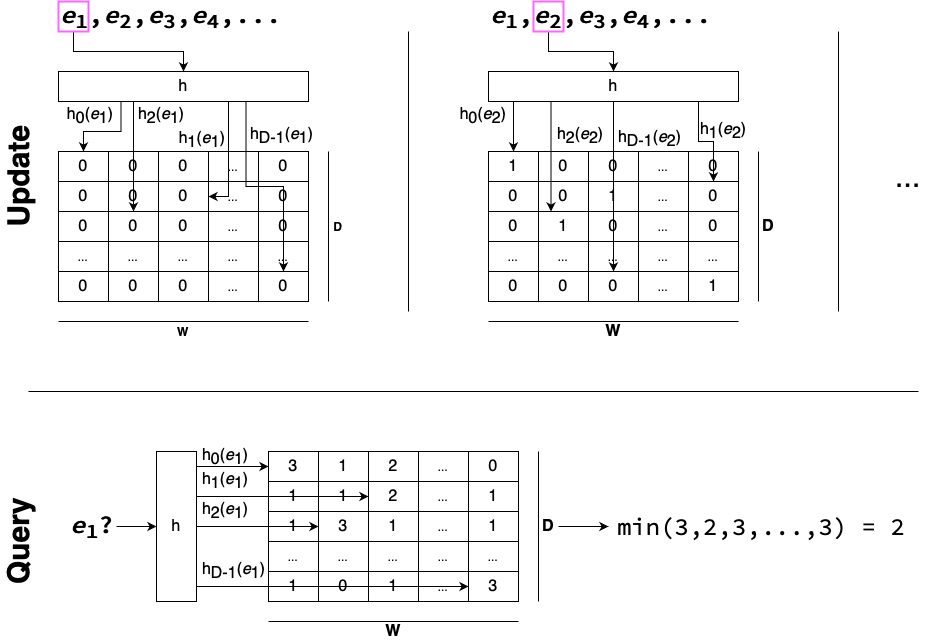
\includegraphics[width=0.8\textwidth]{figures/cm-example}
	\end{center}
	\caption{Example of a \cm sketch being used to count \kmer's. $k=4$}\label{fig:countminexample}
\end{figure}

\subsection{As a representation for a \dBG}

\asq{Vale colocar isso aqui, ou é mais interessante deixar apenas para falar disso no capítulo anterior (State of the Art), quando falando
sobre o \emph{FastEtch}?}

A \cm sketch can implement the membership query operation by querying the count for a given \kmer and comparing it to a presence threshold:
if the count surpasses this threshold, the \kmer is considered to be present in the \dBG, and if the count is inferior to the threshold the
\kmer is considerent absent from the graph.

\section{\dBCM}
\label{sec:debruijncountmin}

% - Representation (what goes in each cell)
% - Operations:
%   - addOutEdge
%   - query 
% - Analysis space/time (may be done within previous sections)

In order to this work we introduce a modified version of the \cm sketch, which we call the \dBCM, that allows the sketch to be queried not only
for \kmer counts, but also for the edges from the \dBG associated with that \kmer. In this way we expect to improve navigability of the
graph through the sketch allowing for the construction of the \dBG online.

In order to store the additional information, we expand the \cm sketch such that each cell in the matrix stores not only the counter,
but also a set of out edges. The structure, then, provides an interface to increment the counters associated with a given key by one,
and an interface to add an out edge to the sets associated with a given key. The increment operation is performed in the same way as in
a regular \cm sketch, and the algorithm for the add edge operation can be seen in Algorithm \ref{alg:addOutEdge}.

Furthermore, the \dBCM must accomodate this new information in its query operation. In order to do this, the sketch returns not only
the minimum value of the counters, but also the intersection of the sets of out edges. The algorithm for the updated query operation is
described in Algorithm \ref{alg:query}.

\begin{algorithm}[htbp]
    \caption{$\mathit{addOutEdge}(\text{k-mer}, \mathit{outEdge})$}\label{alg:addOutEdge}
    \KwData{$\mathit{outEdge} \in \{\A, \C, \G, \T\}$}
    \For{$i = 1, \ldots, D$}{
      $\mathit{CountMin}[i][h_i(\text{k-mer})].\mathit{outEdges} \gets \mathit{CountMin}[i][h_i(\text{k-mer})].\mathit{outEdges} \cup \mathit{outEdge}$\;
    }
\end{algorithm}

From a practical perspectie, due to a node only ever having 4 possible out edges (corresponding to the 4 bases $\{\A, \C, \G, \T\}$),
the set of out edges can be represented by a bit vector indicating whether each of these possible edges is present. An edge is added
by setting the corresponding bit, and the intersection is obtained by performing the bitwise AND operation. This allows both set of
out edges and the counter to be stored together in a single integer.

\begin{algorithm}
    \caption{$\mathit{query}(\text{k-mer})$}\label{alg:query}
    $\mathit{count} \gets \mathit{inf}$\;
    $\mathit{outEdges} \gets \{\A, \C, \G, \T\}$\;
    \For{$i = 1, \ldots, D$}{
      $\mathit{count} \gets \min(\mathit{count}, \mathit{CountMin}[i][h_i(\text{k-mer})].\mathit{count})$\;
      $\mathit{outEdges} \gets \mathit{outEdges} \cap \mathit{CountMin}[i][h_i(\text{k-mer})].\mathit{outEdges}$\;
    }
    \Return{$(\mathit{count}, \mathit{outEdges})$}
\end{algorithm}

\subsection{As a representation of a \dBG}

\section{Hashtable}
\label{sec:debruijnhashtable}
% - Structure
%   - fingerprint
%   - Outedges
% - Hash function 
% - Collision resolution
% - Operations 
%   - Add node/edge
%   - Query node/edge/star 
% - Analysis 

We also propose a new hashtable-based representation for the \dBG that is made more efficient by not storing the \kmer. Instead,
a fingerprint generated from the \kmer is stored, along with the set of out edges as described in Section \ref{sec:debruijncountmin}.
When a \kmer is inserted into the hashtable, or queried from it, a hash value and a fingerprint are calculated in parallel.
In case of an insertion, the fingerprint is written at the desired position and, on a query, the fingerprints are compared. Collisions
are resolved by linear probing, such that if a key tries to insert in a position that is already occupied by a fingerprint that doesn't 
match its own, the \kmer is inserted in the next free position, unless its fingerprint is found before a free position is. During the
query this process is repeated until the desired fingerprint is found, or a free position is reached (in which case the \kmer is
considered to be absent from the structure).

This operation allows for the insertion of a node by adding the \kmer to the hashtable, and the insertion of an edge by updating the
edge set associated with the given \kmer. When queried, the structure returns the edge set associated with the given \kmer, provided
the \kmer has been added to the structure.

\section{A pipeline using the \dBCM and the \dBHT}

% Sequence ---(insert)---> Mod \cm ---(traverse)---> Hashtable 

Beyond the two isolated datastructures to represent the \dBG, we also propose a way to use both of them in tandem in order to obtain
the benefits of both. In this pipeline, the sequencing reads are processed and inserted into the \dBCM as they are made available,
such that the \dBG can be constructed online. Once the reads are all processed in this manner, and a navigatable version of the graph 
has been constructed, it can be traversed, with all of its nodes being, then, inserted in a \dBHT. In this way, a \dBCM is effectively
compressed into a \dBHT.

\section{Experiments}

\subsection{Metrics}

Through the experiments described further in this section, we evaluate different metrics for the \dBCM and the \dBHT. This is due to
the fact that both these structures have different goals and are used in different contexts.

As both of these structures are probabilistic in nature, however, there are certain metrics that are used in the evaluation of both.
One such metric is the \emph{false positive rate}. In this work, we define this rate based on the \kmer's that are visited during a 
traversal of the graph. Let $S$ be a genetic sequence that contains the set of \kmer's $K$, and let $G$ be the graph, represented
either by a \dBCM or a \dBHT, constructed from the sequencing reads of $S$. Further, let $Q$ be the set of \kmer's that were queried
from $G$ during its traversal, and $P={k | k \in Q \wedge k \in G}$ be the set of queried \kmer's that were in $G$. As such, we can
define the set of false positives as $F_P=P \setminus K$ (i.e.: the set of \kmer's that were queried and found to be in $G$ but are not
actually in the original sequence $S$). Finally, the false positive rate is defined as $fp=\frac{|F_P|}{|Q|}$ (i.e.: the ratio of false
positives to the total number of \kmer's that were queried during traversal of $G$).

\asq{Realmente vale a pena tentar fazer isso ainda? Estamos na reta final do projeto já, e isso iria requerer a definição do que é uma
mudança significativa nos resultados que justifique a mudança na estrutura}

Further, as we posit that being able to answer neighborhood queries will improve navigability of the graph by reducing the number of
membership queries made and, thus, the number of false positives, we perform two traversals of the \dBG, the first without using the
out edges information (i.e.: for every node that is in the graph, we query all possible neighboring nodes), and the second with that
information (i.e.: only recorded out edges are used to expand the frontier). We, then, compare the different metrics for the two
traversals.

\subsubsection{\dBCM}

The \dBCM was developed to be used directly with the sequencing reads without any pre-processing. It's goal is to build a reliable
navigatable version of the \dBG as the reads are made available. In this context, not only do we expect a certain amount of false
positives will appear, but as we must probabilistically filter the set of \kmer's from the reads to remove all the spurious ones, we
also expect the occurence of \emph{false negatives}, which are defined as \kmer's from the original sequence $S$ that are not present
in the graph $G$. I.e.: $F_N=K \setminus P$. As such, the \emph{false negative rate} can be defined as the ratio of false negatives
to the total number of \kmer's in the original sequence $S$, or $fn=\frac{|F_N|}{|K|}$.

\subsubsection{\dBHT}

\subsection{\emph{E.~Coli}}

The \emph{E.~Coli} genome is an established benchmark for new assemblers to compare against.

We used the reference genome for the \emph{E.~Coli} bacterium available in \url{http://ftp.ensemblgenomes.org/pub/bacteria/release-52/fasta/bacteria_0_collection/escherichia_coli_str_k_12_substr_mg1655_gca_000005845/dna/}

Three different experiments were performed. In the first we generated simulated perfect reads from the genome by taking substrings of 
the original sequence at random. We then used the \emph{ART Illumina} toolkit \asq{Citation needed} to simulate realistic reads from this
genome, including read errors and reverse complements. Finally, a dataset of real-world reads was downloaded from SRA \asq{Citation Needed}
and used.

\subsubsection{Synthetic reads without errors}

Given the reference genome $S$, the length of each read, $L$, and the desired coverage $C$, the synthetic reads were generated by picking
$\frac{|S| \times C}{L}$ substrings of $S$ at random. This is presented in algorithmic form in Algorithm \ref{alg:generate-reads}.

\begin{algorithm}
  \caption{Generate Reads}\label{alg:generate-reads}
  \KwData{$S$, the reference genome, $L$ the read length, $C$ the coverage}
  $\mathit{\#reads} \gets \frac{|S| \times C}{L}$\;
  $reads \gets \emptyset$\;
  \For{$i \gets 1, \ldots, \mathit{\#reads}$}{
    $j \gets \mathit{random}(0, |S| - L)$\;
    $\mathit{reads.add}(S[j: j+L])$\;
  }
  \Return{$reads$}
\end{algorithm}

\subsubsection{Synthetic reads with errors}

In order to simulate the reads as they would be produced by the sequencing process, we used the ART Illumina toolkit to generate
synthetic reads from the \emph{E.~Coli} genome. The reads were generated using the following parameters:

\begin{enumerate}
\item \textbf{Sequencing System}: Illumina MiSeq v3
\item \textbf{Read length}: \textit{250bp}
\item \textbf{Coverage}: \textit{80x}
\end{enumerate}
    \chapter{Results}

\section{Theoretical Results}\asq{bad name}

\asq{This feels like it should be in methodology?}

Relationship between $c$, $t$, and $W$: a false positive occurs when $C.\mathit{query}(X).c - f(X) \geq t$, so we set $\epsilon F < t \rightarrow \epsilon < \frac{t}{F}$ in order to use Equation~\ref{eq:cm-prob} to establish a false positive rate. Because of the relationship $W = \frac{2}{\epsilon}$, we can put $W$ in terms of $t$: $W > \frac{2F}{t}$. Finally, we expect $F \approx c \times |\strname{S}|$, such that $W > \frac{2 \times c \times |\strname{S}|}{t}$.

Considering that there are approximately $2 \times |\strname{S}|$ distinct real \kmer{s} (including the reverse complements), we would use close to \asq{Close to because $W > \frac{2 \times c \times |\strname{S}|}{t}$, and here I'm considering $W =  \frac{2 \times c \times |\strname{S}|}{t}$} $\frac{c}{t} \times D \times 16$ bits per \kmer. It is clear, therefore, that using a higher value of $t$ is, theoretically, more space-efficient. Using $D = 8$ for an expected false positive rate of $\delta = 0.004$, and setting $t = \frac{c}{2}$, we expect to need 256 bits per \kmer. In this scenario, the \dBG for the \emph{E.~Coli} genome, with nearly 4.6Mb, would be represented in close to 147MB of memory. The human genome would need just over 200GB.

In practice we will show that this is an overestimate, as the sketch seems to perform better than expected.

\asq{Is it possible to create an expression for the false positive rate during traversal? It would depend on (a) the chance that a false \kmer is added to the starting set (so the chance that a false \kmer that appears at the beginning of a read is considered high-frequency) and (b) the chance that a real \kmer has a false edge pointing to a false \kmer}

\section{The \dBCM as a \dBG representation}

We started by evaluating how well the \dBCM performs the task of \kmer counting, comparing the distribution of frequencies, and observing the average error. However, because the goal of this data structure is to allow categorization of \kmer{s} as high- or low-frequency, more than obtaining exact \kmer counts, we take a special interest in evaluating how much the miscounts impact in differentiation between the two categories. To do this, we categorize the \kmer{s} according to a series of thresholds $t$, using both the exact frequency for each \kmer and the frequency estimated by the \dBCM. Let $H$ be the set of \kmer{s} categorized as high-frequency, and $K$ be the set of \kmer{s} found in the reference genome \strname{S} and its reverse complement \strname{\overline{S}}. We then generate $F_P = H \setminus K$, the set of spurious \kmer{s} that were considered to be high-frequency (false positives), and $F_N = K \setminus H$, the set of true \kmer{s} that were not considered to be high-frequency (false negatives). By analysing how the sizes of these sets varies as a function of $t$ we find the optimal threshold for differentiating the two categories.

Because the parameter $W$ has an important impact on the magnitude of the expected overcount, we analyze how they affect the error by comparing the mean and standard deviation for this metric accross varying values of $W$.

We have used $D = 8$ as it gives a high degree of confidence in Equation~\ref{eq:cm-prob} (0.04\% chance of a miscount being greater than $\epsilon F$).

We selected an initial value of $W$ by estimating $t = 40$ as a good threshold value due to it being equidistant from the expected frequency of real \kmer{s} ($80$), and of spurious \kmer{s} ($1$). We then made $W = \frac{2F}{t} = 20M$. The distributions of the exact frequencies and those estimated by the resulting \dBCM sketch are presented side-by-side in Figure~\ref{fig:ecoli-art-frequencies}. We can see that the estimated frequencies are shifted right in relation to the exact frequencies, expected from the fact that the \dBCM will err by overcounting. However, we can see that the distribution remains clearly bimodal. Therefore, it is possible to choose a value $t$ that divides the \kmer{s} into the two categories.

\begin{figure}[htbp]
    \centering
    \begin{subfigure}{.5\textwidth}
        \centering
        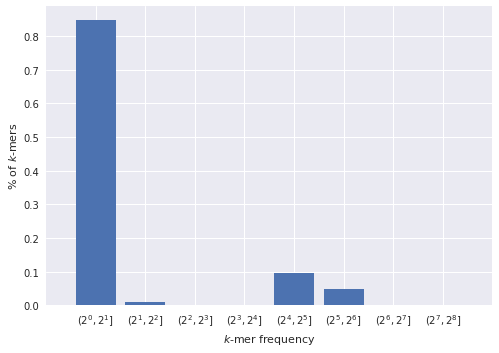
\includegraphics[width=\textwidth]{figures/e_coli-kmer_frequencies-exact-K31}
        \caption{Exact frequencies}\label{fig:ecoli-art-frequencies-exact}
    \end{subfigure}%
    \begin{subfigure}{.5\textwidth}
        \centering
        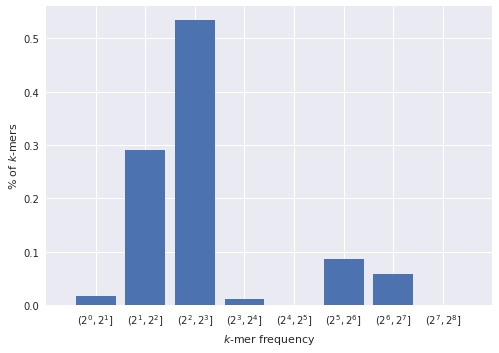
\includegraphics[width=\textwidth]{figures/e_coli-kmer_frequencies-estimated-K31-W20000000}
        \caption{Estimated frequencies}\label{fig:ecoli-art-frequencies-estimated}
    \end{subfigure}
	\caption{\kmer frequencies for \emph{E.~Coli} genome with $k=31$. \dBCM parameters: $(W=20M, D=8)$}\label{fig:ecoli-art-frequencies}
\end{figure}

Using the same count results, we selected values of $t \in \{1, 10, 20, \ldots, 160 (2 \times c)\}$ and compared the percentages of the true \kmer{s}, and of the spurious \kmer{s}, that were considered high-frequency. Figure~\ref{fig:ecoli-art-thresholds} presents the results when we use the exact counts for categorizing next to the results from using the estimated counts. Firstly, we can see that, when using either exact or estimated count, $t = 10$ is enough to filter out the majority of spurious \kmer{s}, further demonstrating that most of them appear a very low number of times in the reads. Moreover, we can see that the range of $t$ for which almost all real \kmer{s} are considered to be high-frequency is widened by using the estimated counts. This is to be expected, again, due to collisions and overcounting. Likewise, we see that $t$ must also be higher before we see the number of false \kmer{s} categorized as high-frequency diminish.

\begin{figure}[htbp]
    \centering
    \begin{subfigure}{.5\textwidth}
        \centering
        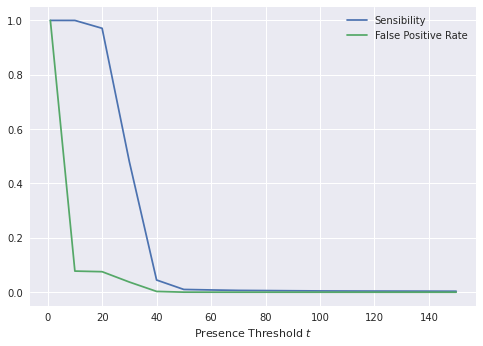
\includegraphics[width=\textwidth]{figures/e_coli-threshold_exploration-K31-exact}
        \caption{Exact counts}\label{fig:ecoli-art-threshold-exact}
    \end{subfigure}%
    \begin{subfigure}{.5\textwidth}
        \centering
        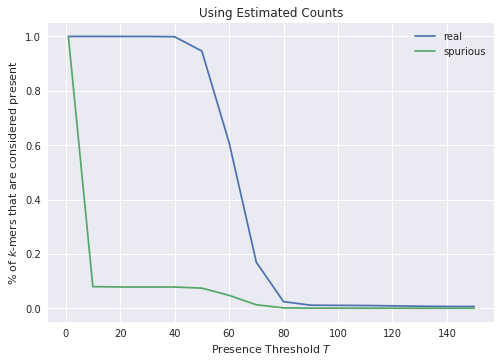
\includegraphics[width=\textwidth]{figures/e_coli-threshold_exploration-K31-W20000000-D8}
        \caption{Estimated by \dBCM ($W=20M, D=8$)}\label{fig:ecoli-art-frequencies-W20000000-D8}
    \end{subfigure}
    % \begin{subfigure}{.5\textwidth}
    %     \centering
    %     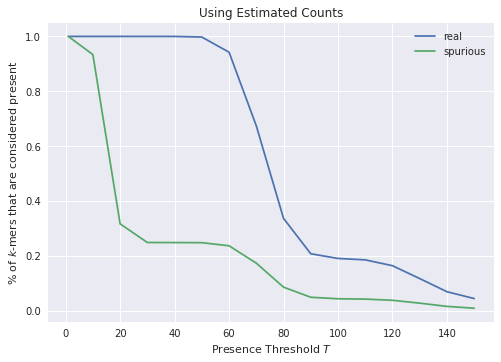
\includegraphics[width=\textwidth]{figures/e_coli-threshold_exploration-K31-W7500000-D8}
    %     \caption{Estimated by \dBCM ($W=7.5M, D=8$)}\label{fig:ecoli-art-frequencies-W7500000-D8}
    % \end{subfigure}
	\caption{Percentages of true and spurious \kmer{s} considered to be high-frequency according to different values of $t$ using (a) exact and (b) estimated counts (\dBCM parameters: $(W=20M, D=8)$).}\label{fig:ecoli-art-thresholds}
\end{figure}

We, then, iteratively lowered $W$ to evaluate how smaller sketches performed in \kmer counting, seeing how this affected the mean error, as well as the standard deviation. The results are seen in Figure~\ref{fig:ecoli-art-error}, where we plot the mean and standard deviation of the count errors as a function of $W \in \{5M, 7.5M, \ldots, 17.5M, 20M\}$. Because the spurious \kmer{s} appear a low number of times, analysing the mean error, as well as the standard deviation of the errors gives good insight into what kind of threshold would be needed to successfully categorize the \kmer{s} according to frequency, as we expect $50\%$ of \kmer{s} to have its count overestimated by the mean error or less, and over $80\%$ of \kmer{s} \toconsider{should} have a count that is overestimated by the mean plus one standard deviation. By analizing Figure~\ref{fig:ecoli-art-error}, we can see that there is little increase in the mean and standard deviation of the error from $W = 20M$ to $W = 10M$, with performance deteriorating much more quickly after that.

One interesting thing to note is that, with $W = 10M$, both the mean and the standard deviation of the error are below $20$, such that we expect over $80\%$ of the \kmer counts to not be overestimated by more than $40$. In fact, in Section~\ref{sec:traversal-results} we show that the \dBCM performs very well with $t = 40$ and $W = 10M$, half of the size suggested by Equation~\ref{eq:cm-prob}.

\begin{figure}[htbp]
    \centering
    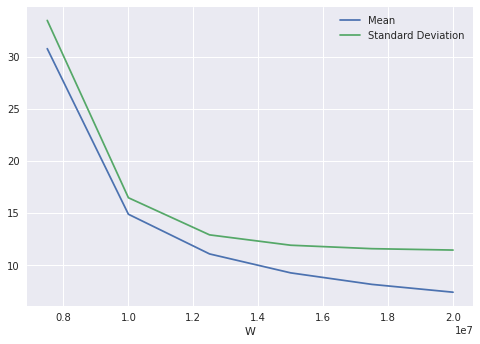
\includegraphics[width=0.9\textwidth]{figures/e_coli-error_mean_stddev-K31-D8-T40}
    \caption{Error mean and standard deviation as a function of $W$}\label{fig:ecoli-art-error}
\end{figure}

In Figure~\ref{fig:ecoli-art-W7500000} we replicate the results of the \dBCM from Figures~\ref{fig:ecoli-art-frequencies}~and~\ref{fig:ecoli-art-thresholds} for $W = 7.5M$, showing the other extreme of the range. \asq{Passar por aqui de novo, mas para mostrar o outro lado da range o correto seria mostrar $W = 5M$, e $W = 7M$ já apresenta um erro significativamente maior de forma que para representar o extremo ainda positivo, faria mais sentido usar $W = 10M$.}

\begin{figure}[htbp]
    \centering
    \caption{}\label{fig:ecoli-art-W7500000}
\end{figure}

\asq{Falar aqui sobre diminuir $D$?}

\asq{Teria sido possivel gerar algum valor que não seja o erro ou o desvio padrão que permita definir o quão bem aquele valor de $W$ consegue dividir os \kmer{s} nas duas categorias? Algo tipo: fazer a variação do $t$ e aí encontrar o $t$ que maximiza a diferença entre o percentual de \kmer{s} reais inclusos e o percentual de \kmer{s} espúrios, e aí usar essa diferença de percentual para determinar o quão bem aquele valor de $W$ consegue diferenciar as duas categorias?}

\subsection{Memory Usage}

We can express the number of bits per \kmer needed to represent the \dBG allowing for an expected false positive rate---the chance that a spurious \kmer will be considered high-frequency---$\delta$ in terms of the sequencing coverage $c$, and the presence threshold $t$ to be used. The total memory used is $16 \times W \times D$ bits, and we expect there to be $|\strname{S}|$ distinct \kmer{s} in the sequence. Because we add \kmer{s} both in forward and reverse complement direction, approximately $2 \times |\strname{S}|$ distinct \kmer{s} are represented in the \dBG. Benefiting from the fact that the majority of spurious \kmer{s} appear only once or twice in the reads, we can consider that they will only be considered high-frequency when they are miscounted by almost $t$. As such, we can express the false positive rate as $\prob[C.\mathit{query}(X) - f(X) > t]$, and use Equation~\ref{eq:cm-prob} to establish a relation between the size of the \dBCM, determined by $W$ and $D$, and the false positive rate in terms of $t$ by making $\epsilon F = t$. Because $F \approx c \times |\strname{S}|$, we can express $W = \frac{2 \times c \times |\strname{S}|}{t}$, while $D = \log(\frac{1}{\delta})$ remains the same. The total size of the \dBCM, then, is $16 \times \frac{2 \times c \times |\strname{S}|}{t} \times \log(\frac{1}{\delta})$ bits. Since we expect around $2 \times |\strname{S}|$ distinct \kmer{s} to be represented in the \dBG, we arrive at approximately $16 \times \lceil \frac{c}{t} \rceil \times \lceil \log(\frac{1}{\delta}) \rceil$ bits per \kmer. Choosing $t = \frac{c}{2}$ and a desired false positive rate of $1\%$, we expect the \dBCM to need $147$ bits per \kmer.

\asq{Um problema sério dessa sessão é que, na prática, a taxa de falsos positivos vai ser mais alta do que o valor definido. Isso acontece porque existe uma quantidade de \kmer{s} espúrios que tem um contagem maior do que 1 ou 2, de forma que a garantia de $C.\mathit{query}(X) - f(X) \leq t$ é uma garantia fraca. Para eliminar esses \kmer{s} seria necessário definir o erro máximo aceito como um valor menor do que o threshold de presença (i.e. $C.\mathit{query}(X) - f(X) \leq t - \beta$). Não sei se tem alguma forma de definir esse valor de forma sistemática (e.g. qual é o menor threshold para o qual, baseado na contagem real, esperamos cortar $90\%$ dos \kmer{s} espúrios?) Talvez seja possível chegar a tal expressão baseado na probabilidade do erro, e a probabilidade de dois erros distintos gerarem o mesmo \kmer, mas acredito que seria uma expressão complexa.}

\section{Traversal of the \dBCM}
\label{sec:results-dbcm-traversal}

The previous results suggest that the \dBCM is possibly an apt representation of the \dBG as an MDS, with its expected false positive rate for $W = 20M$ being below $20\%$, as can be extrapolated from the percentage of spurious \kmer{s} categorized as high-frequency. Although not ideal, it is likely not high enough to \toconsider{disrupt} usage of the graph \cite{Pell2012}. However, we expect the addition of outedges to improve on the navigability of the graph, resulting in an even lower false positive rate in practice, as the graph is traversed.

To test this, we traversed the \dBCM starting from a set of known member nodes selected during construction of the graph by picking the first \kmer of each read if its count already surpassed $t$. During traversal, we register all the \kmer{s} that are queried from the \dBCM (which we call $Q$), as well as the query result. With this data, we evaluate how many \kmer{s} are queried during traversal, and how many of those are actually found to be in the graph (we refer to the set of \kmer{s} found during traversal as $V$). We can, then, define the set of false positives $F_P = V \setminus K$ and the set of false negatives as $F_N = K \setminus V$. We establish the false positive rate as $f_p = \frac{|F_P|}{|V|}$ and the false negative rate as $f_n = \frac{|F_N|}{|K|}$.

\asq{Aqui vale colocar alguns resultados e gráficos para uma instância específica (talvez $W = 20M$ de novo), como, por exemplo, a distribuição do número de arestas em cada nó visitado. Isso deve permitir entender o porque de a taxa de falsos positivos crescer tão rapidamente aparentemente de repente.}

Figure~\ref{fig:ecoli-art-traversal-W-queriedfound} presents the number of \kmer{s} queried and found during traversal for different \dBCM with different parameters $W$ \asq{Importante notar que são usados os mesmos valores de $W$ que antes, exceto por $W = 5M$, que foi excluído porque, devido a alta taxa de falsos positivos, o programa estoura a memória e é interrompido sem gerar resultados}. Figure~\ref{fig:ecoli-art-traversal-W-fpfn} shows the false positive and false negative rates as a function of $W$.

\begin{figure}[htbp]
	\centering
    \begin{subfigure}{.5\textwidth}
        \centering
        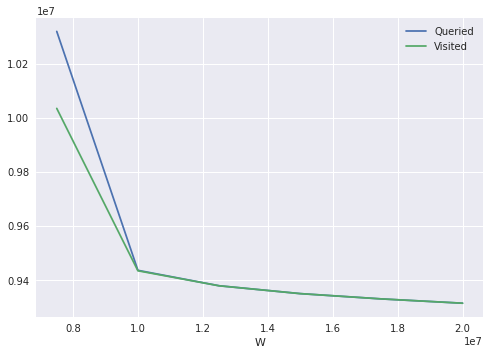
\includegraphics[width=\textwidth]{figures/e_coli-dbcm-queried_and_found-K31-D8-T40}
        \caption{Queried \& Found}\label{fig:ecoli-art-traversal-W-queriedfound}
    \end{subfigure}%
    \begin{subfigure}{.5\textwidth}
        \centering
        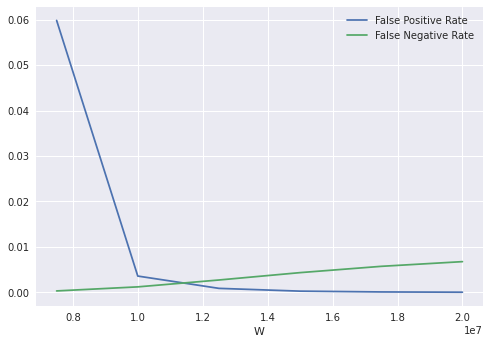
\includegraphics[width=\textwidth]{figures/e_coli-dbcm-false_positive_and_negative_rates-K31-D8-T40}
        \caption{False Positives}\label{fig:ecoli-art-traversal-W-fpfn}
    \end{subfigure}
	\caption{Number of (a) \kmer{s} queried and found during traversal and (b) false positives}\label{fig:ecoli-art-traversal-W}
\end{figure}

\section{Construction of the \dBHT from the \dBCM}

\asq{Trazer informações aqui sobre o tempo necessário para a construção da nova estrutura}

\section{Traversal of the \dBHT}

\asq{Trazer os mesmos gráficos da Seção~\ref{sec:results-dbcm-traversal} sendo que para a \dBHT. Falar sobre como ela tem uma taxa de falsos positivos maior do que a \dBCM, apesar de apenas os nós visitados na \dBCM serem adicionados na \dBHT e as arestas ainda passarem por uma limpeza (arestaas que não apontam para um nó real no \dBCM não são adicionadas na \dBHT). Isso provavelmente acontece porque usar 8 hashes distintos previne mais colisões do que apenas um hash e um fingerprint.}
    \chapter{Conclusion}

\section{\cm{-based} \kmer counting can be used to filter spurious \kmer{s} from sequencing reads}

We expand on the results presented by Zhang \emph{et al.} \cite{Zhang2014} to show that despite overcounting, we can still filter out most (over $80\%$) of spurious \kmer{s} based on the count estimate from a \cm sketch that has fewer cells, in total, than the number of distinct \kmer{s} in the reads, and uses only $16$ bits per cell. These results are similar to what \emph{khmer} achieves through iteratively truncating the reads at the first low-frequency \kmer \cite{Zhang2014}, i.e. \emph{read trimming}. However, filtering directly from the counts only requires that the reads be processed one time.

\section{Filtering through traversal is very effective}

We have also shown that traversing the \dBG generated from the high-frequency \kmer{s} further improves filtering of spurious \kmer{s} without affecting the number of real \kmer{s} represented. Therefore, although Ghosh \& Kalyanaraman \cite{Ghosh2019} present a framework for using the \cm sketch for online filtering of spurious \kmer{s} that allows the sketch to be considerably smaller, reducing the size of the \cm sketch much further than presented here hinders its ability to be successfully navigated, losing a very efficient second filter that removed nearly $98\%$ of the remaining spurious \kmer{s} after count-based filtering. This would decrease memory requirement during processing of the reads, but results in a less succint representation of the \dBG.

\section{Storing outedges improve traversal}

We also see that, for both data structures used, the number of outedges stored for each node in the \dBG is low, with the vast majority having only one recorded outedge. Without using the outedges, and querying all four possible outneighbors of a given node, we would need to query between $2$ and $4\times$ as many \kmer{s}, just from the nodes represented in the \dBG. Storing the outedges, even with some chance of false positives, can, therefore, decrease the impact of the false positive rate associated with the membership query of either structure by stopping false \kmer{s} from ever being queried. Moreover, by reducing the number of queries that need to be made, storing the set of outedges also improves time-performance of traversal.

\section{\dBHT can succesfully represent a \dBG in as few as $9$ bits per \kmer}

Finally, we have shown that the \dBHT can represent a \dBG in as few as $9$ bits per \kmer with, at most, $16\%$ of the graph being composed of false \kmer{s} introduced by the probabilistic nature of the representation. Based on the exploration by Pell \emph{et al.} \cite{Pell2012}, we expect this number of false positives not to affect usability of the graph for assembly. We can reduce it, however, by increasing the size of the \dBHT. With $16$ bits per \kmer, we achieved a number of false positive nodes that is below $4\%$ of the total number of \kmer{s} represented in the graph.

These results are comparable to current \dBG representations, that span from $4$ bits per \kmer to $24$ bits per \kmer \cite{Chikhi2013} \cite{Giani2020}.

\section{Future Works}

\subsection{Directly compare against similar works}

It is important to compare the results obtained in this work against similar works. Notably, we would like to show that the \cm{-based} filter used in \emph{FastEtch} is less effective in filtering spurious \kmer{s} than the filtering pipeline we introduce, based on count and traversal. We would also like to show that despite providing a slightly less succint \dBG representation in the form of a \dBHT, this representation presents better performance than Bloom Filter based representations, due to both reducing the number of queries needed by avoiding the need to query all four neighbors of a node, as well as by reducing the number of hashing functions used to only two (hashing and fingerprint).

\subsection{Generating contigs and N50 score for the \dBHT}

A natural next step is to use the \dBHT to generate maximal contigs and, from them, generate the N50 score, a metric defined as the length $l_0$ of the shortest contig such that all contigs with length $l \geq l_0$ cover at least $50\%$ of the assembly. The N50 score is used to determine que quality of an assembly in terms of contiguity. Based on the distribution of outedges observed during traversal of the \dBHT, we expect this representation to perform fairly well.

\subsection{Use \dBHT as visited set during traversal of \dBCM}

To traverse the \dBCM, we have used both a queue to store the nodes that should be visited, and a set to store the nodes that have been visited.In practice, this approach is not interesting as it ultimately requires representing the \dBG in memory as a set, in parallel to the succint representation being constructed, which is prohibitive in larger genomes. Although a representation that is more succint than a set, but less so than the \dBHT could be used, it would be interesting to see how using the \dBHT, as it is being constructed, as the set of visited nodes would affect its final results. Because the \dBHT allows for false positives, we expect some probability that a node will be considered to already have been visited in traversal, and, therefore, its outedges might not be represented in the graph. This could, in the best case, potentially lead to further filtering and, in the worst case, cause loss in sensitivity, as the main component of the \dBG is broken up.

    \backmatter
    \bibliographystyle{abbrv}
    \bibliography{references}
\end{document}
